\documentclass{article}
\usepackage[T1]{fontenc}
\usepackage{lmodern}
\usepackage{graphicx}
\usepackage{amsmath,amssymb}
\usepackage[a4paper,margin=2cm]{geometry}
\usepackage[absolute,overlay]{textpos}
\setlength{\TPHorizModule}{1mm}
\setlength{\TPVertModule}{1mm}
\usepackage[indonesian]{babel}
\usepackage{hyperref}
\setlength{\emergencystretch}{2em}
% unit: Halaman 35

\begin{document}

% === Halaman 35 (llm) ===

\vspace{145.53mm}

Stego-image
\vspace{20mm}
Extracted image

\vspace{109.89mm}

% deskripsi: Gambar stego yang menampilkan seekor rubah salju di tengah salju putih.
% bbox normalisasi: [0.1500, 0.0200, 0.5500, 0.5100]
\begin{textblock*}{84.00mm}(31.50mm,5.94mm)
\noindent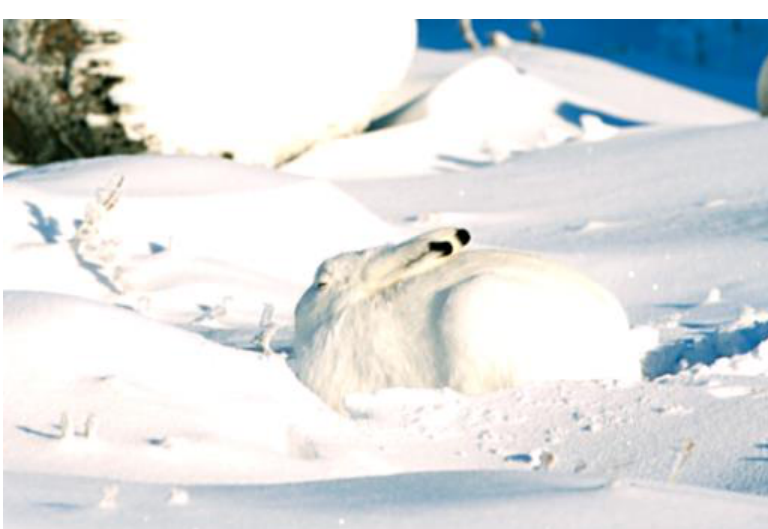
\includegraphics[width=84.00mm,height=145.53mm]{../../images/llm/page_035_img_01.png}%
\end{textblock*}

% deskripsi: Gambar yang diekstraksi menampilkan sebuah jet tempur yang sedang terbang.
% bbox normalisasi: [0.5100, 0.5300, 0.8300, 0.9000]
\begin{textblock*}{67.20mm}(107.10mm,157.41mm)
\noindent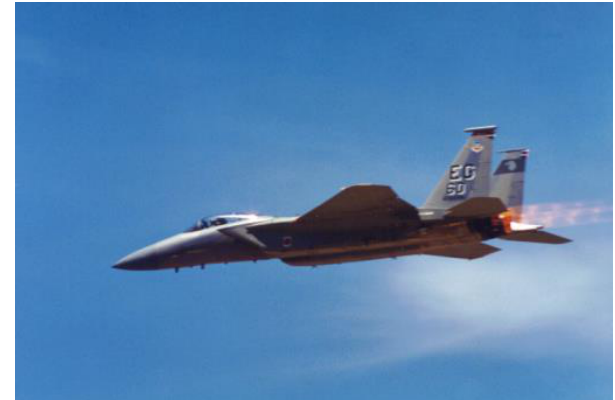
\includegraphics[width=67.20mm,height=109.89mm]{../../images/llm/page_035_img_02.png}%
\end{textblock*}

\end{document}
